\section{Human Object Tracking} \label{sec:track}
After abstracting the blob masks into feature vector representation shown in \autoref{eq:blobdenote2}, the tracking algorithm finally comes into use. To handle the one-to-many relation between blobs and actual objects, we introduce an abstract layer called object layer above the observed blob layer. The tracking algorithm maintains a list of known objects and matches an object with its optimum pair in the blob list given by the feature extractor. Every object consists of the attributes listed in \autoref{tab:objectattributes}.

 Overall speaking, the objective of the tracking layer is to:
\begin{enumerate}
  \item track the blobs by their centroid as much as possible
  \item if step 1 fails, try matching existing object with one of the central points
  \item in step 2, choose the most likely candidate for matching among all central points, considering the previous object location, motion direction as well as speed, as mentioned in \autoref{sec:featureextract}
  \item determine if two blobs actually belong to one previous object, as mentioned in \autoref{sec:detect}
  \item determine if it is an entering/ exiting event by an object's first position and last seen position, as well as modify the room occupancy count
\end{enumerate}

The above listed tracking steps are adapted from \cite{sharma2012blob} for a top-view IR image sequence, and could be further divided to two phases.

In the pairing phase, the location of an object will be updated to the paired blob location with a filter. If an object cannot find a suitable blob pair, it will not be eliminated immediately but continue propagated a few frames with the previous velocity to see if there could be a match on the forward trajectory. This is exactly the virtual track method used by \cite{virtualtrack}.

If there is at least one unmatched blob left in the blob list, the spawn phase is activated. The tracking algorithm first check if the matched blob could be a fraction of a splitted blob. If it is the case, the blob will be merged to the nearby existing object and contribute to the object location update. Finally, if the blob is unlikely to have any relation with existing objects, a new object will be spawned from the blob center.
\begin{table}
  \centering
  \begin{tabular}{|c|c|}
    \hline
    % after \\: \hline or \cline{col1-col2} \cline{col3-col4} ...
    i & unique label \\
    $\vec{x}$ & current position \\
    $\vec{\dot{x}}$ & current velocity \\
    $\vec{x_0}$ & position of first appearance \\
    $t_v$ & number of virtual track propagation \\
    \hline
  \end{tabular}
  \caption{Object attributes for tracking}\label{tab:objectattributes}
\end{table}

\subsection{Matching step}
The objects and blobs are matched by a distance score based on nearest neighbour rule. By matching, a time disparity between the objects and blobs should be considered. Because the blobs are observed at a time step $t$, but the object location are updated in the last time step $t-1$. By the time of matching, the objects should have already moved forward. Therefore, the blobs should be matched with the \emph{predicted position} of the objects.

A Kalman filter could be used to store the object states and predict its next state by state transition \cite{mika,virtualtrack}. Since the states in our use case only contains two components (position and velocity), and the second one is the derivative of the first one, an Alpha-Beta filter could be used to simplify the filtering process and cutdown unnecessary computational overhead.

An Alpha-Beta filter resembles Kalman filter in its nature, combining state transition and observation for state update, but does not vary coefficients dynamically. Denote $\hat{\boldmath{x}}$ as the estimated value, $\boldmath{x}^p$ as the predicted value and $\boldmath{x}^m$ as the measured value, the system state is obtained by the following \autoref{eq:abfilter}.
\begin{equation}\label{eq:abfilter}
  \left\{
  \begin{split}
    & \hat{\boldmath{x}}_n = \boldmath{x_n}^p + \alpha\left(\boldmath{x_n}^m-\boldmath{x_n}^p\right)\\
    & \hat{\boldmath{\dot{x}}}_n = \boldmath{\dot{x}}^p_n + \frac{\beta}{T}\left(\boldmath{x_n}^m-\boldmath{x_n}^p\right)\\
    & \boldmath{x_{n+1}}^p = \hat{\boldmath{x}}_n + T \hat{\boldmath{\dot{x}}}_n\\
    & \boldmath{\dot{x}_{n+1}}^p = \boldmath{\dot{x}_{n}}
  \end{split}
  \right.
\end{equation}

In the first two lines of \autoref{eq:abfilter}, $\alpha$ and $\beta$ are two fixed coefficients that are chosen experimentally. For an camera installed at a height of 2.5m with a FOV of $60^\circ C$, we choose $\alpha=0.75,\ \beta=0.8$. \autoref{fig:trackexample1} demonstrates the smoothen effect of the filter, the estimated trajectory becomes more stable compared to the measured trajectory. More importantly, even though the filter uses fixed coefficients, the prediction usually approximate the actual measurement very well. An exception is when the human moves close to the border, because the human body is only partially detected, the centroid of that partial body stays almost still. The estimated object position will converge quickly to the actual (but wrong) measurement. This behaviour is designed intended so that the tracking could be continued. 

During the middle stem of the trajectory when the human is fully observed, the predicted position given by the filter largely simplifies the tracking algorithm. The distance threshold between a blob observation and an object no longer depends on the object velocity, but merely on the prediction deviation and measurement error. Therefore, the distance threshold could be reduced to a low value, which potentially avoids false matching because of a large searching radius. 

Moreover, an (relatively) accurate prediction could solve the nearest neighbour issue during central point matching mentioned in \autoref{sec:featureextract}. By central points extraction, several points on the child branch would be inevitably picked to be possible candidates, while the actual blob central must locate on the main branch. Since those points on the child branch are closer to the border therefore closer to the last estimated object location, they will have a higher chance in paring if we directly match the last estimated object location with the measurement. However, with one time step forward prediction, the predicted object location will locate approximately on the main branch of the central point representation, and the tracking algorithm will choose a candidate that is closer to the actual object position.

For both centroid matching and central points matching, we choose a distance threshold of 15 pixels. This value is chosen based on the camera installation height and normal walking speed.

\begin{figure}
  \centering
  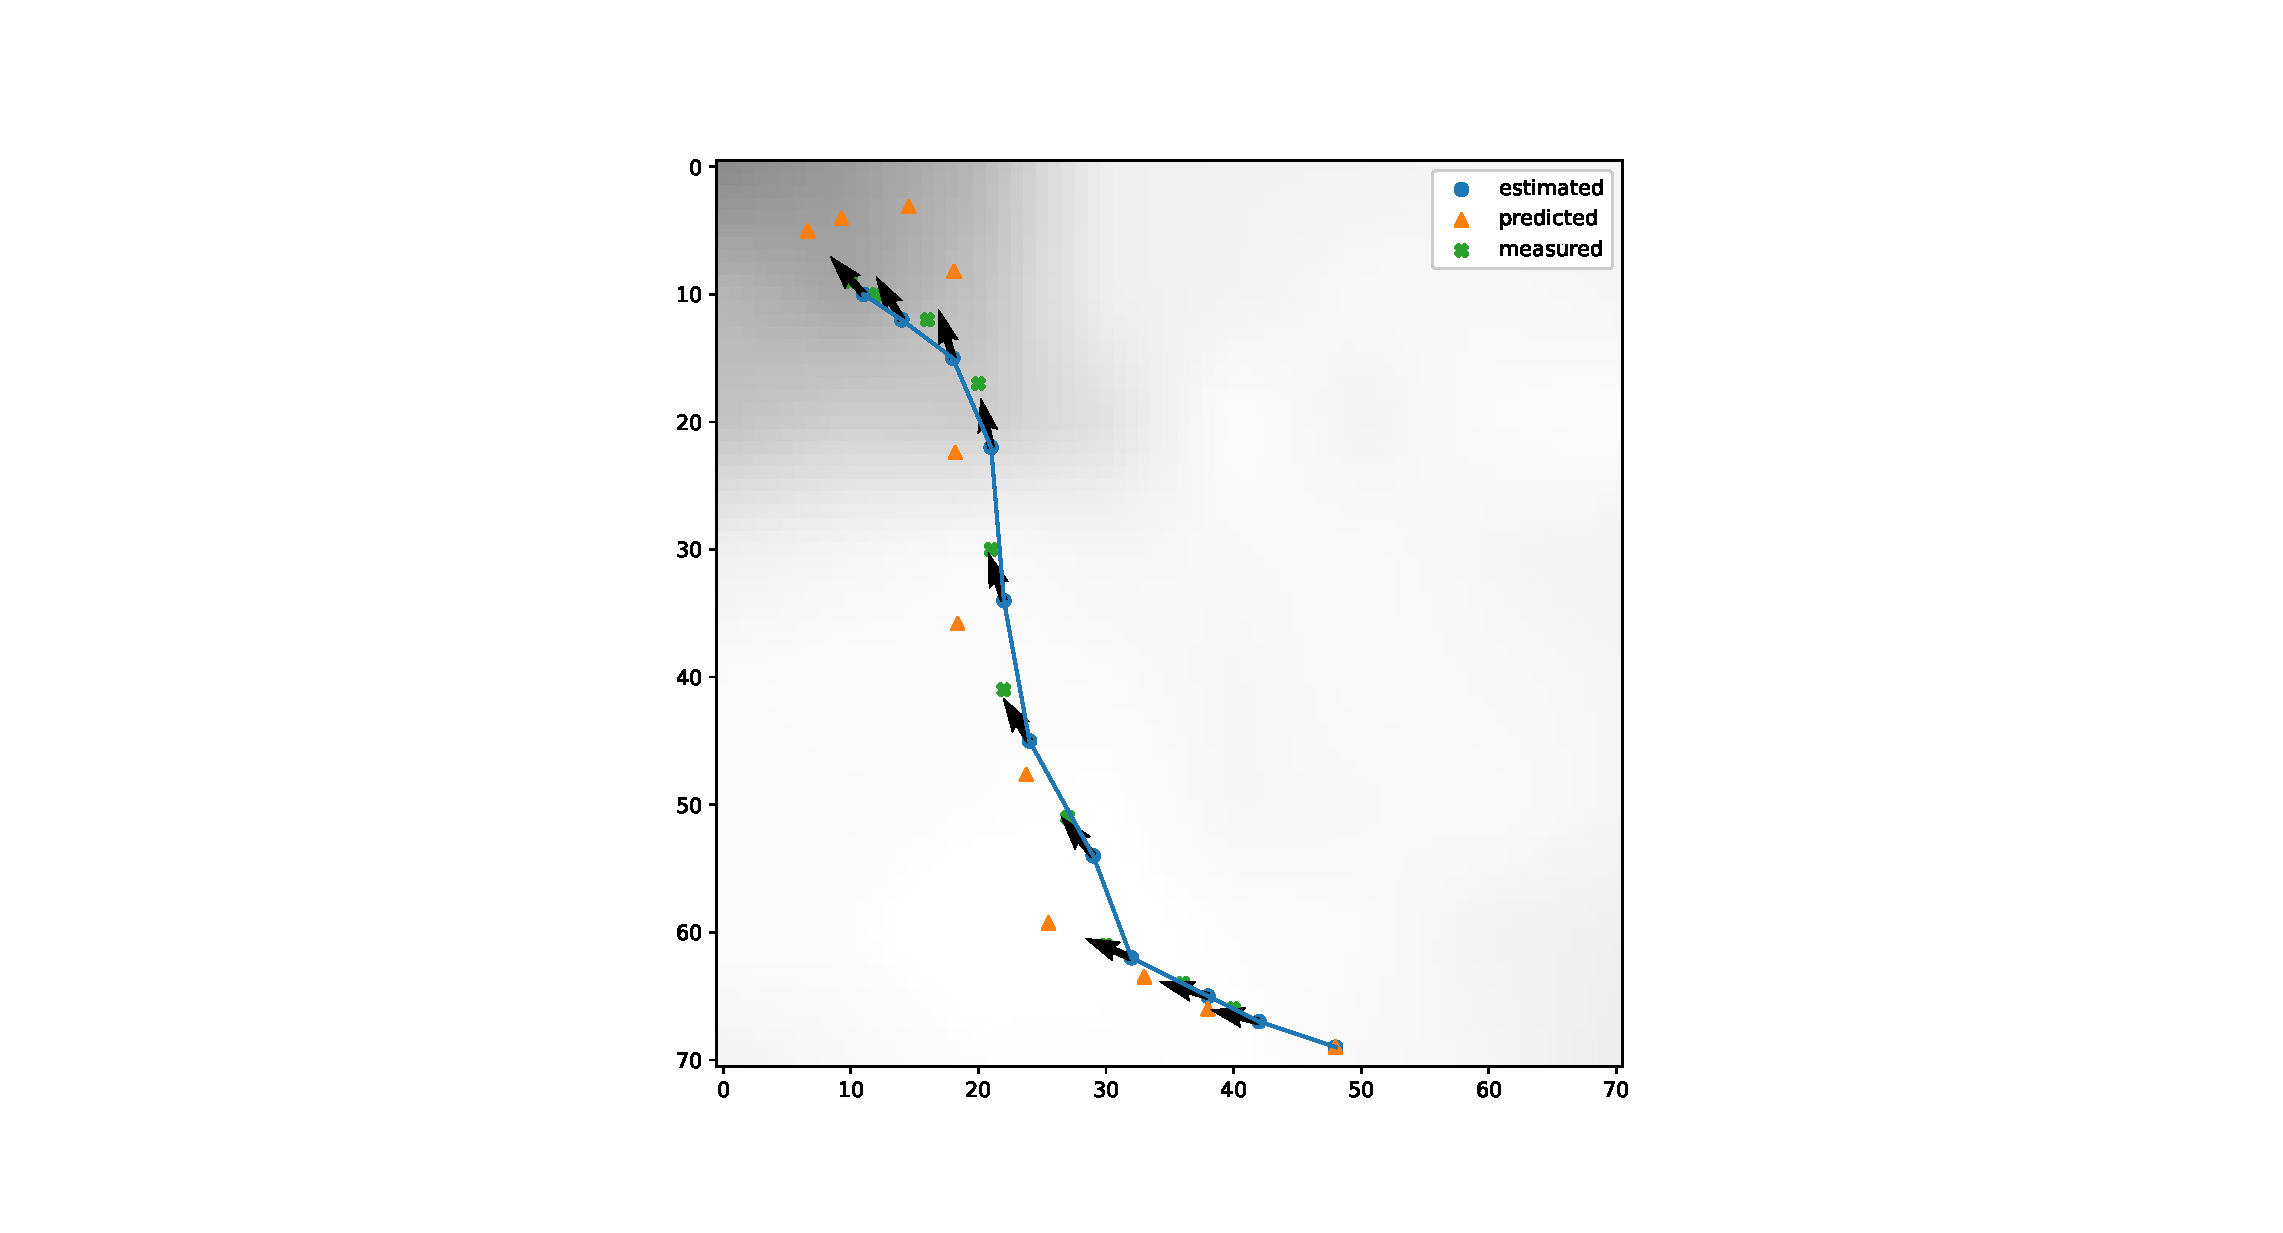
\includegraphics[width=\textwidth]{figures/trackexample1.eps}
  \caption{A track example. The blue dot shows the estimated position, the quiver from the blue dot points the velocity direction of the object and the yellow triangle shows the predicted position one time step forward.}\label{fig:trackexample1}
\end{figure}
\begin{figure}
  \centering
  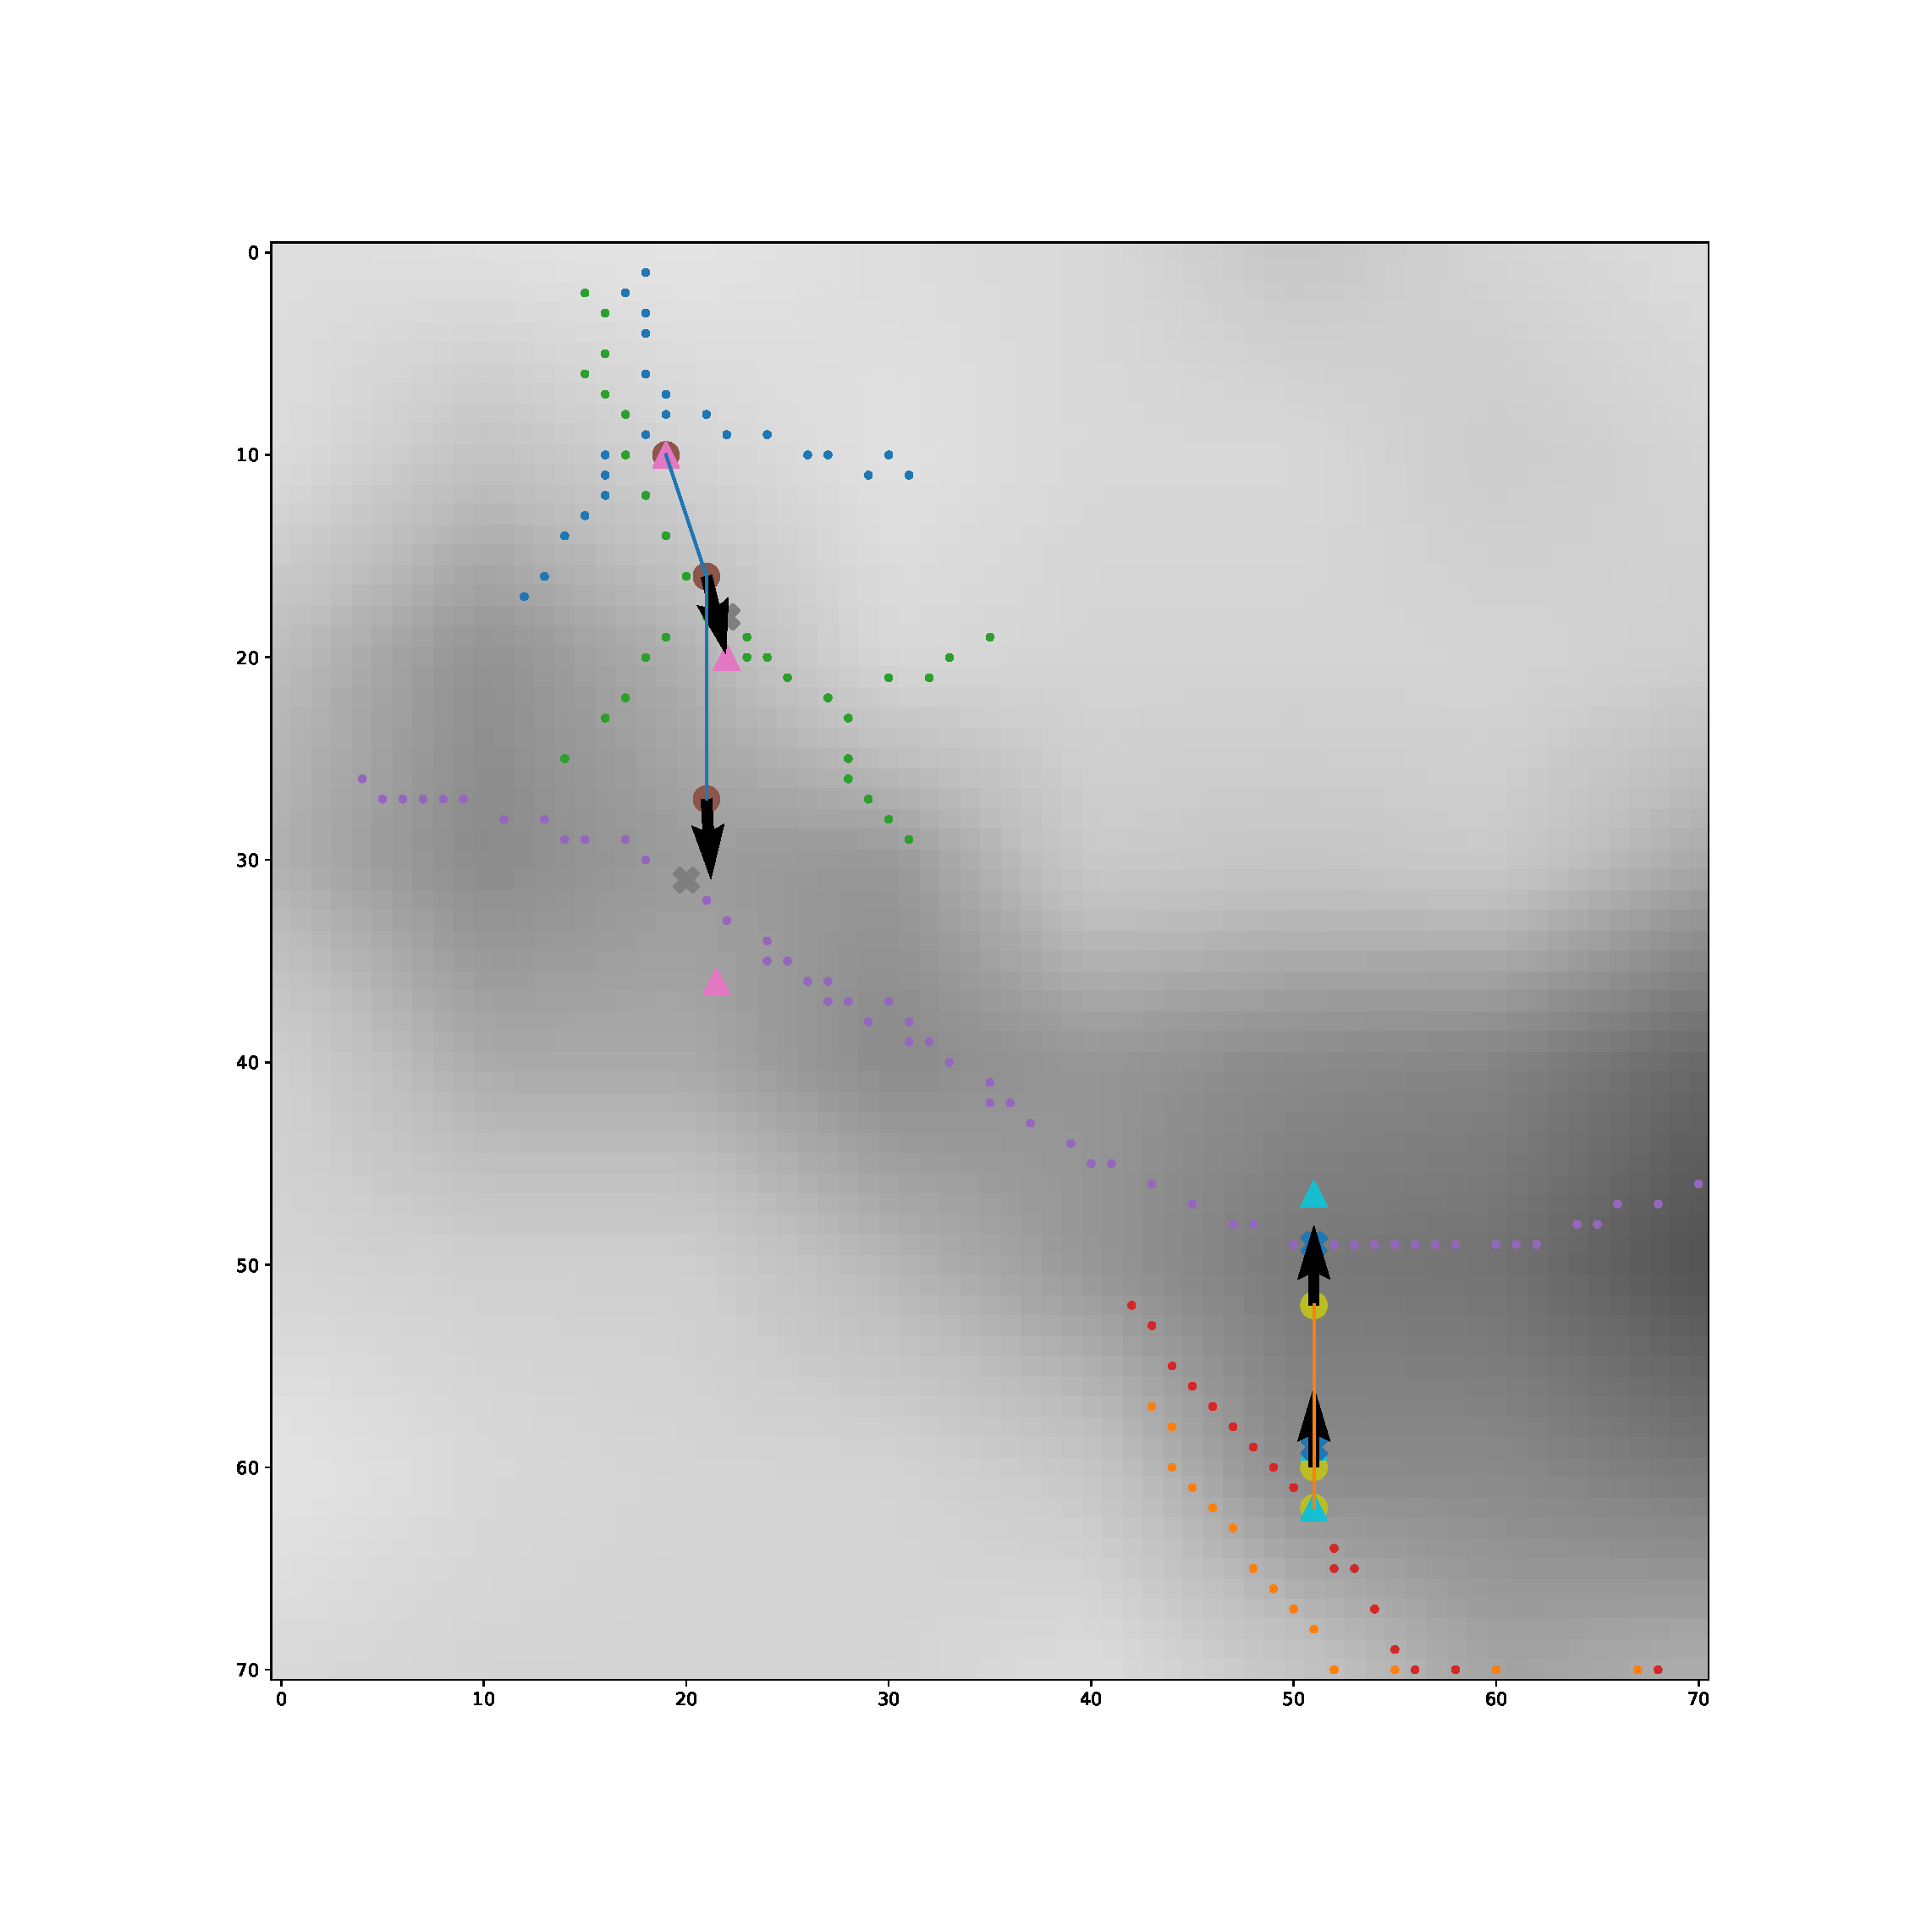
\includegraphics[width=\textwidth]{figures/trackexample2.eps}
  \caption{A track example (same sequence as \autoref{fig:blobmerge}) until two blobs merged and the central point matching is activated. The pixel dots represent the central points. The round markers are the estimated object location, triangle markers are prediction, and cross markers are measurements. Blob contour is omitted for a clear demonstration.}\label{fig:trackexample2}
\end{figure}
\begin{figure}
  \centering
  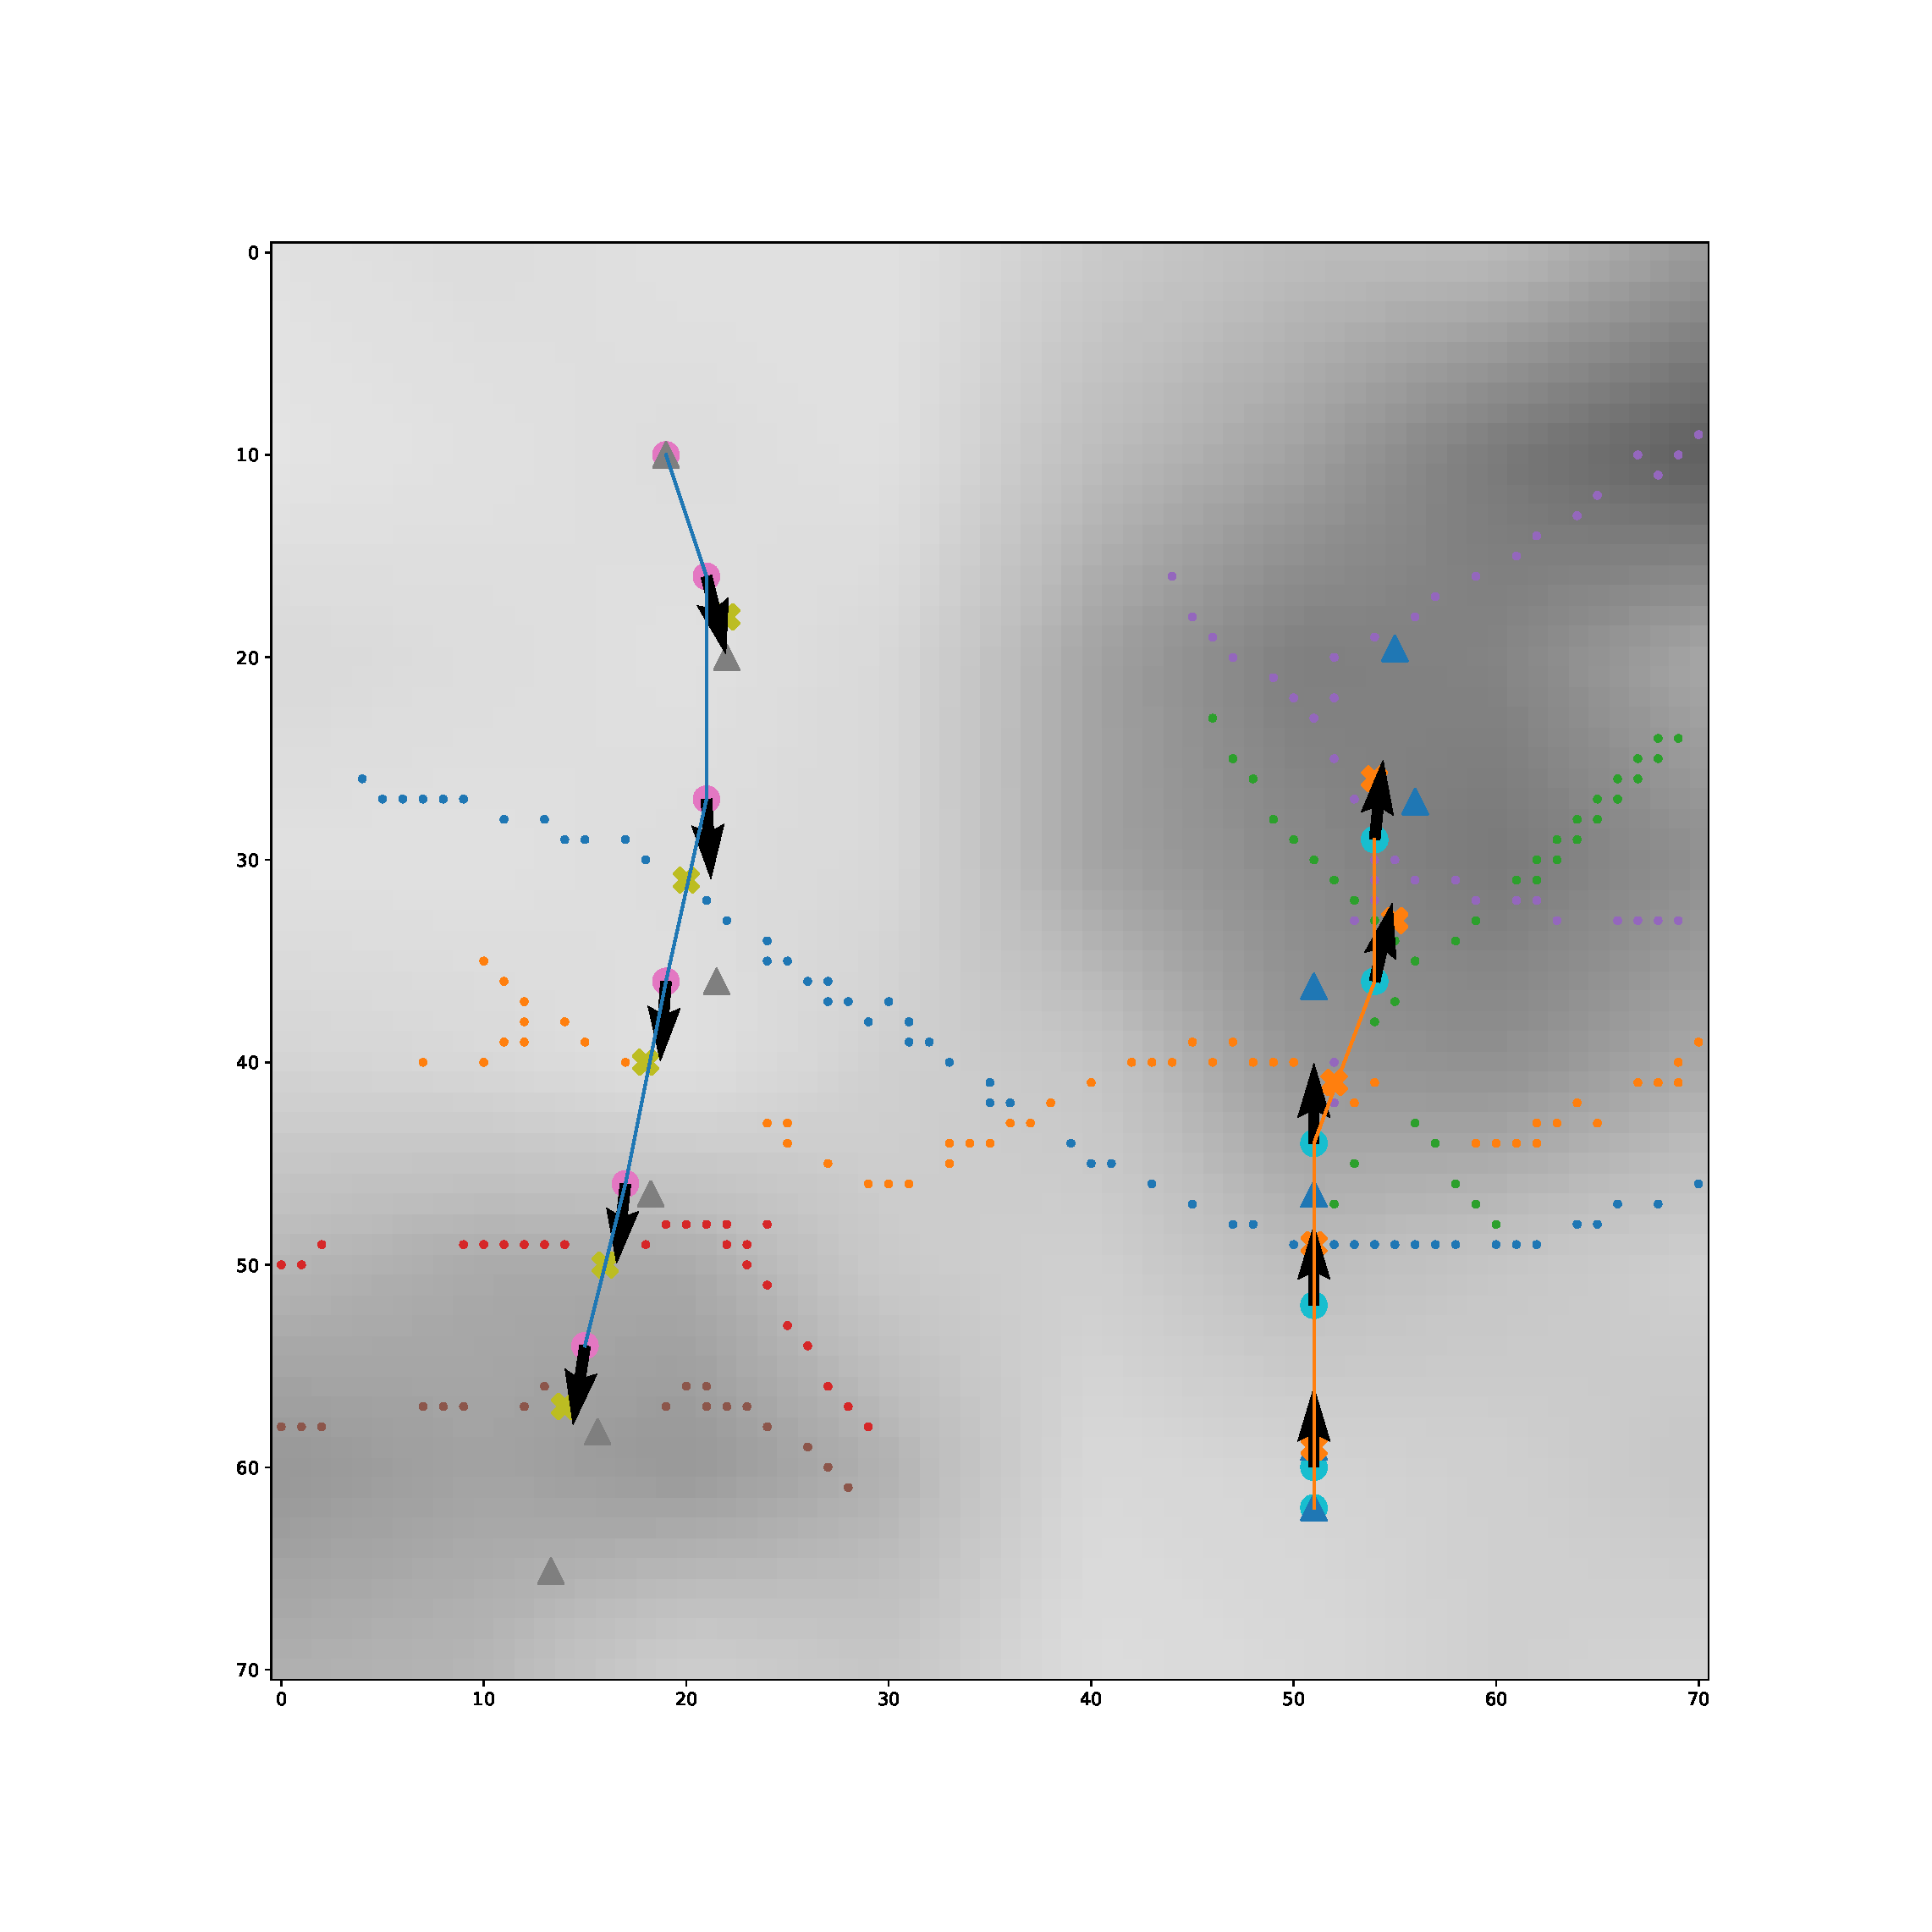
\includegraphics[width=\textwidth]{figures/trackexample2_2.eps}
  \caption{A track example (same sequence as \autoref{fig:blobmerge}, continued from \autoref{fig:trackexample2}) after the merge event. The tracking algorithm successfully handle the merging blobs correctly and continue tracking with centroids.}\label{fig:trackexample2_2}
\end{figure}

\subsection{Virtual track}
\subsection{Blob registration}

